% Rowley-Brooke et al. (CVPR 2013) vs our modified pipeline, stage by stage.
% Same conventions as pipeline.tex. Paper row uses only equations written in the paper.
% Build: tectonic bleed/diagrams/comparison.tex
\documentclass[border=8pt]{standalone}
\usepackage{amsmath,amssymb,bm}
\usepackage{tikz}
\usetikzlibrary{shapes.arrows,positioning,shadows,fit,calc}

\definecolor{blockedge}{HTML}{7FA7D9}
\definecolor{navy}{HTML}{1F3B73}
\definecolor{hl}{HTML}{FFF2A8}
\definecolor{none}{HTML}{F1F1F1}

\tikzset{
  blk/.style={draw=blockedge, line width=0.9pt, fill=white, text width=6.7cm, minimum height=3.5cm,
              align=center, drop shadow={opacity=0.22, shadow xshift=0.6mm, shadow yshift=-0.6mm}},
  harrow/.style={single arrow, draw=black, fill=white, line width=0.6pt, minimum height=1.05cm,
                 single arrow head extend=0.12cm, inner sep=1.6pt},
}
\newcommand{\ttl}[2]{\textcolor{navy}{\bfseries\Large #1}\\\textcolor{navy}{\bfseries\Large #2}}
\newcommand{\note}[1]{\\[3pt]\mbox{\small\color{black!70}#1}}
\newcommand{\hollow}[2]{%
  \path let \p1=(#1), \p2=(#2), \n1={veclen(\x2-\x1,\y2-\y1)} in
    node[harrow, minimum height=\n1, anchor=tail] at (#1) {};}

\begin{document}
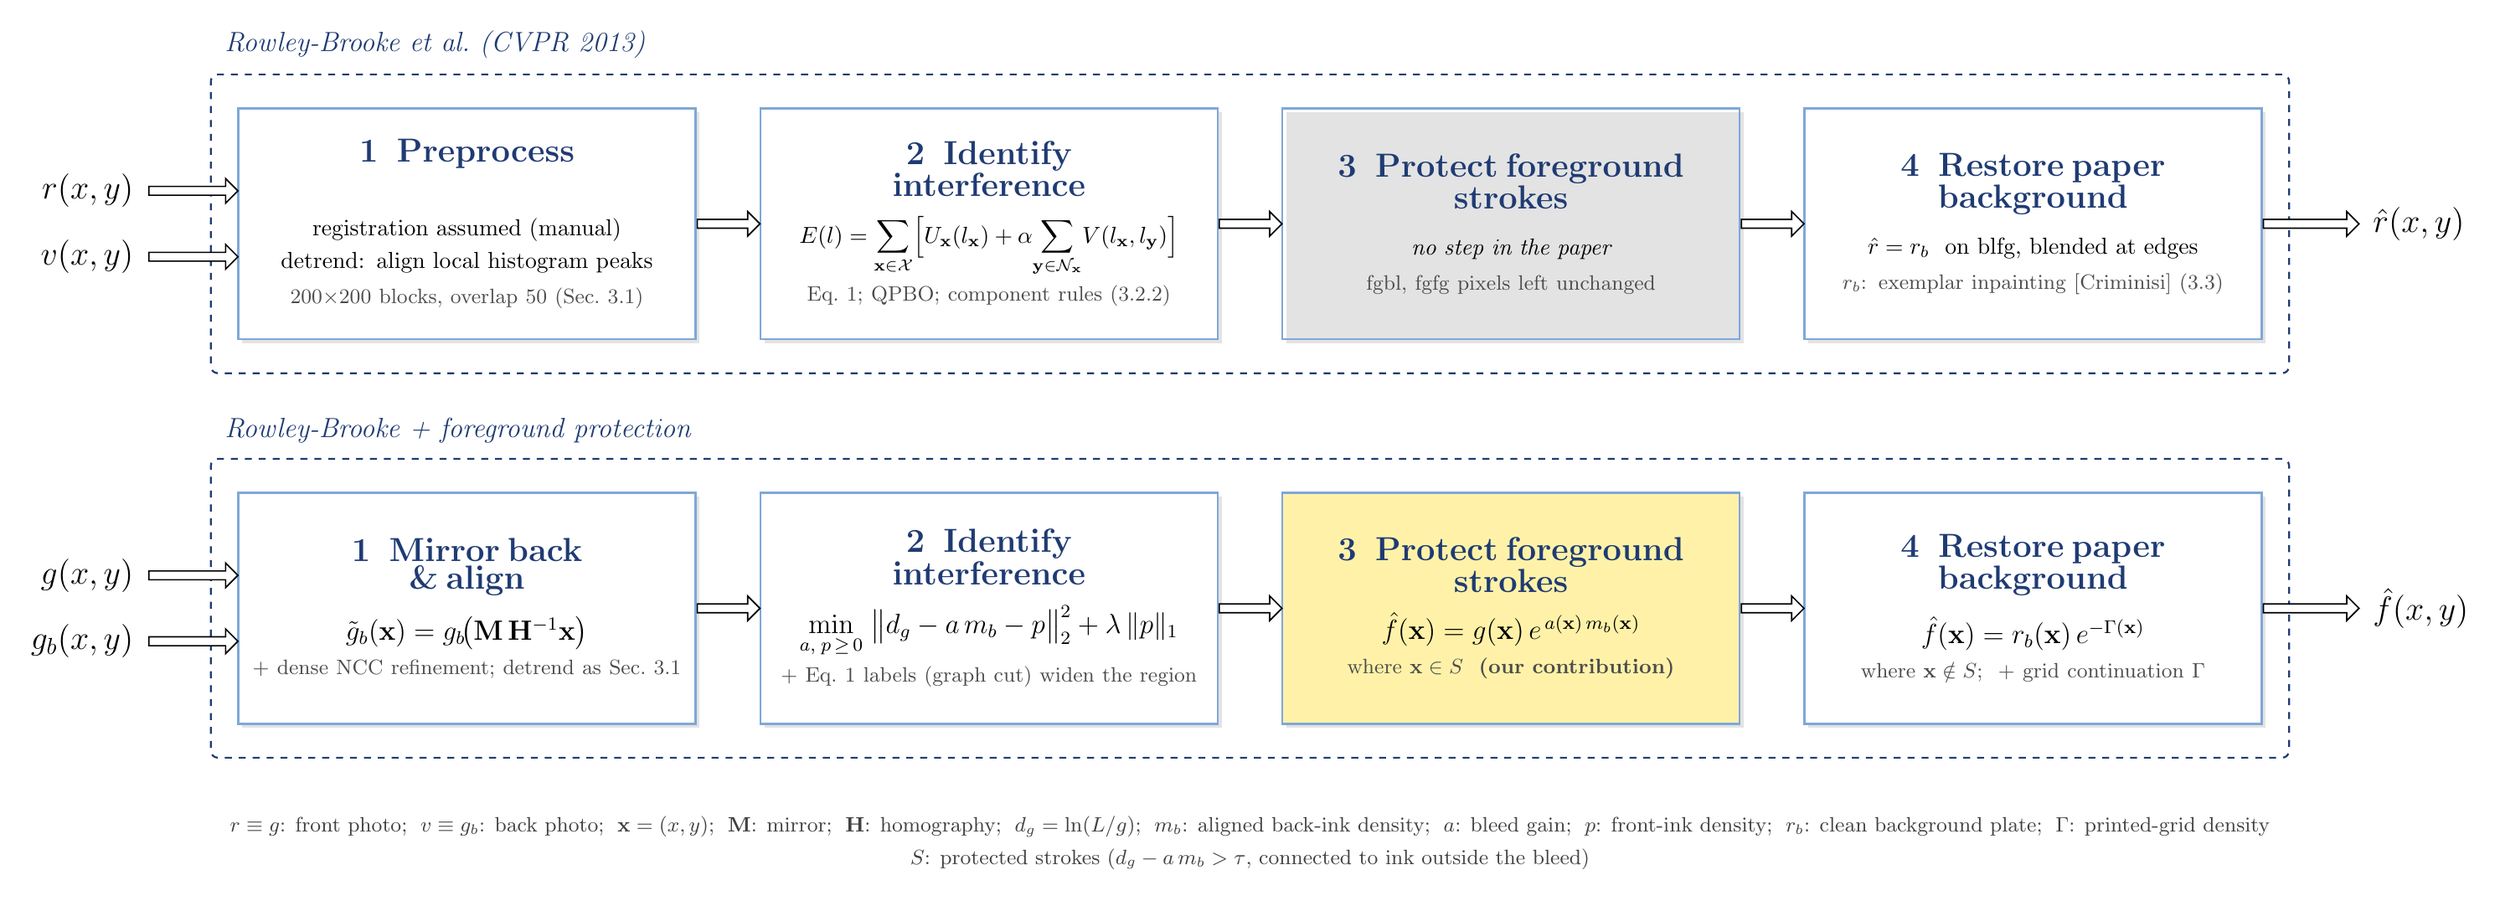
\begin{tikzpicture}[node distance=0.95cm and 0.95cm]
  % ---------------- Rowley-Brooke et al. 2013 ----------------
  \node[blk] (p1) {\ttl{1\enspace Preprocess}{\phantom{g}}\\[8pt]
      \mbox{registration assumed (manual)}\\[2pt]
      \mbox{detrend: align local histogram peaks}\note{200$\times$200 blocks, overlap 50 (Sec.\ 3.1)}};
  \node[blk, right=of p1] (p2) {\ttl{2\enspace Identify}{interference}\\[8pt]
      \mbox{$\displaystyle E(l)=\sum_{\mathbf{x}\in\mathcal{X}}\Bigl[U_{\mathbf{x}}(l_{\mathbf{x}})
            +\alpha\!\sum_{\mathbf{y}\in\mathcal{N}_{\mathbf{x}}}\!V(l_{\mathbf{x}},l_{\mathbf{y}})\Bigr]$}
      \note{Eq.\ 1; QPBO; component rules (3.2.2)}};
  \node[blk, right=of p2, fill=none] (p3) {\ttl{3\enspace Protect foreground}{strokes}\\[8pt]
      \mbox{\itshape no step in the paper}\note{fgbl, fgfg pixels left unchanged}};
  \node[blk, right=of p3] (p4) {\ttl{4\enspace Restore paper}{background}\\[8pt]
      \mbox{$\hat{r}=r_b$\ \ on blfg, blended at edges}
      \note{$r_b$: exemplar inpainting [Criminisi] (3.3)}};

  % ---------------- Ours ----------------
  \node[blk, below=2.3cm of p1] (o1) {\ttl{1\enspace Mirror back}{\& align}\\[8pt]
      \mbox{\large$\tilde{g}_b(\mathbf{x}) = g_b\!\bigl(\mathbf{M}\,\mathbf{H}^{-1}\mathbf{x}\bigr)$}
      \note{+ dense NCC refinement; detrend as Sec.\ 3.1}};
  \node[blk, right=of o1] (o2) {\ttl{2\enspace Identify}{interference}\\[8pt]
      \mbox{\large$\displaystyle\min_{a,\;p\,\ge\,0}\;\bigl\lVert d_g - a\,m_b - p\bigr\rVert_2^2 + \lambda\,\lVert p\rVert_1$}
      \note{+ Eq.\ 1 labels (graph cut) widen the region}};
  \node[blk, right=of o2, fill=hl] (o3) {\ttl{3\enspace Protect foreground}{strokes}\\[8pt]
      \mbox{\large$\hat{f}(\mathbf{x}) = g(\mathbf{x})\,e^{\,a(\mathbf{x})\,m_b(\mathbf{x})}$}
      \note{where $\mathbf{x}\in S$\ \ \textbf{(our contribution)}}};
  \node[blk, right=of o3] (o4) {\ttl{4\enspace Restore paper}{background}\\[8pt]
      \mbox{\large$\hat{f}(\mathbf{x}) = r_b(\mathbf{x})\,e^{-\Gamma(\mathbf{x})}$}
      \note{where $\mathbf{x}\notin S$;\ \ + grid continuation $\Gamma$}};

  % groups
  \node[draw=navy, dashed, line width=0.8pt, rounded corners=3pt, inner xsep=0.4cm, inner ysep=0.5cm,
        fit=(p1)(p4)] (gp) {};
  \node[anchor=south west, font=\itshape\large, text=navy] at ([xshift=1mm, yshift=1mm]gp.north west)
        {Rowley-Brooke et al.\ (CVPR 2013)};
  \node[draw=navy, dashed, line width=0.8pt, rounded corners=3pt, inner xsep=0.4cm, inner ysep=0.5cm,
        fit=(o1)(o4)] (go) {};
  \node[anchor=south west, font=\itshape\large, text=navy] at ([xshift=1mm, yshift=1mm]go.north west)
        {Rowley-Brooke + foreground protection};

  % inputs / outputs
  \foreach \row/\a/\b/\out in {p/r/v/\hat{r}, o/g/g_b/\hat{f}} {
    \node[anchor=east, align=left] (\row in1) at ([xshift=-1.45cm, yshift= 0.5cm]\row1.west) {\Large $\a(x,y)$};
    \node[anchor=east, align=left] (\row in2) at ([xshift=-1.45cm, yshift=-0.5cm]\row1.west) {\Large $\b(x,y)$};
    \node[anchor=west] (\row out) at ([xshift=1.55cm]\row4.east) {\Large $\out(x,y)$};
  }
  \foreach \row in {p, o} {
    \hollow{$(\row in1.east)+(0.1,0)$}{$(\row1.west|-\row in1.east)$}
    \hollow{$(\row in2.east)+(0.1,0)$}{$(\row1.west|-\row in2.east)$}
    \hollow{\row1.east}{\row2.west}
    \hollow{\row2.east}{\row3.west}
    \hollow{\row3.east}{\row4.west}
    \hollow{\row4.east}{$(\row out.west)+(-0.1,0)$}
  }

  % key
  \node[below=0.75cm of go.south, align=center] {%
    {\small\color{black!75}$r\equiv g$: front photo;\; $v\equiv g_b$: back photo;\; $\mathbf{x}=(x,y)$;\;
     $\mathbf{M}$: mirror;\; $\mathbf{H}$: homography;\; $d_g=\ln(L/g)$;\; $m_b$: aligned back-ink density;\;
     $a$: bleed gain;\; $p$: front-ink density;\; $r_b$: clean background plate;\; $\Gamma$: printed-grid density}\\[2pt]{\small\color{black!75}$S$: protected strokes ($d_g-a\,m_b>\tau$, connected to ink outside the bleed)}};
\end{tikzpicture}
\end{document}
